\chapter{Kajian Pustaka}
\label{chapter:kajian-pustaka}

Bab ini akan diisi oleh kajian pustaka yang berkaitan dengan topik persoalan tugas akhir untuk memberikan informasi mengenai dasar teori dan studi yang dipakai. Bab ini diharapkan dapat membantu pembaca untuk lebih mengerti tentang penelitian tugas akhir ini.

\section{Teknik \textit{Scaling} Basis Data Relasional}

Terdapat berbagai teknik umum yang digunakan untuk melakukan \textit{scaling} pada basis data relasional. Berikut adalah beberapa di antaranya:

\subsection{Replikasi basis data}

Replikasi berarti menyimpan salinan data yang sama pada beberapa mesin yang berbeda dan terhubung melalui jaringan \parencite{dataIntensiveApplications}. Terdapat beberapa alasan mengapa hal ini lazim dilakukan, yaitu:

\begin{enumerate}
    \item Untuk menjaga data tetap dekat secara geografis kepada pengguna, sehingga latensi berkurang.
    \item Agar sistem dapat terus berjalan meski terjadi kegagalan pada sebagian sistem, sehingga \textit{availability} meningkat.
    \item Untuk melakukan \textit{scale out} banyaknya mesin yang bisa melayani \textit{read queries}, sehingga meningkatkan \textit{read throughput}.
\end{enumerate}

Salah satu pendekatan yang umum diimplementasikan pada basis data relasional seperti PostgreSQL adalah replikasi berbasiskan \textit{leader and follower}. Satu \textit{node} ditugaskan sebagai \textit{leader} yang menerima operasi \textit{read and write}, lalu setiap perubahan yang terjadi akan direplikasi oleh replika (\textit{follower}). Dengan pola seperti ini, umumnya operasi \textit{write} hanya dapat ditangani oleh \textit{leader} dan operasi \textit{read} dapat ditangani oleh semua \textit{node}.

\begin{figure}[ht]
    \centering
    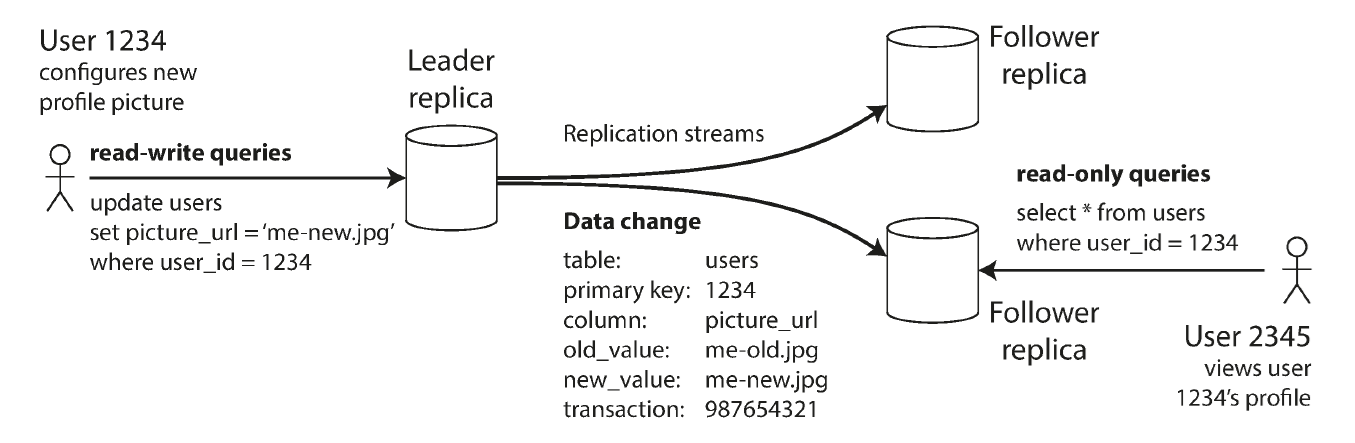
\includegraphics[width=0.8\textwidth]{resources/chapter-2/leader-based-replication.png}
    \caption{\textit{Leader-based (master-slave) replication \parencite{dataIntensiveApplications}}}
    \label{fig:leader-based-replication}
\end{figure}

Selain itu, proses replikasi juga terbagi menjadi dua, yaitu \textit{synchronous replication} dan \textit{asynchronous replication}. Pada \textit{synchronous replication}, data yang akan ditulis juga harus sudah ditulis oleh semua (atau mayoritas) replika sebelum dapat di-\textit{acknowledge}. Pada \textit{asynchronous replication}, data akan ditulis terlebih dahulu pada \textit{leader} lalu perubahannya dipropagasikan kepada \textit{replika}. Setiap pendekatan ini memiliki \textit{tradeoff} tersendiri. \textit{Synchronous replication} menjamin mayoritas \textit{node} memiliki data paling terbaru, tetapi latensi pada proses penulisan akan meningkat, sedangkan pada \textit{asynchronous replication} latensi penulisan jauh lebih kecil, tetapi data pada \textit{replica} menjadi \textit{eventually consistent}. Kedua mode replikasi ini didukung oleh PostgreSQL.

\section{\textit{Event-Driven Architecture}}

\textit{Event-driven architecture} merupakan paradigma arsitektur perangkat lunak yang berkaitan dengan produksi dan deteksi \textit{event}. Arsitektur ini mudah dievolusikan dan menawarkan toleransi kegagalan (\textit{fault tolerance}), kinerja yang baik, dan pemskalaan yang baik. Meskipun begitu, arsitektur ini kompleks dan sulit untuk diuji. Arsitektur ini cocok untuk kasus yang kompleks dan dinamis \parencite{softwareArchitecture}.

Arsitektur ini terdiri atas tiga komponen, yaitu \textit{event producer}, \textit{event router}, dan \textit{event consumer}. Sebuah produsen mengirimkan \textit{event} ke \textit{router}, lalu disaring dan dikirimkan kepada konsumen.

\subsection{Redpanda}

Redpanda merupakan \textit{event streaming platform}. Platform ini menyediakan infrastruktur untuk \textit{streaming real-time data}. Produsen mengirimkan data berupa \textit{event} ke Redpanda, kemudian Redpanda menyimpan \textit{event} tersebut lalu mengaturnya ke dalam sebuah topik. Topik ini merupakan log \textit{event} yang dapat diputar ulang. Konsumen mengonsumsi \textit{event} pada topik Redpanda secara asinkron \parencite{redpandaIntro}.

\begin{figure}[htbp]
    \centering
    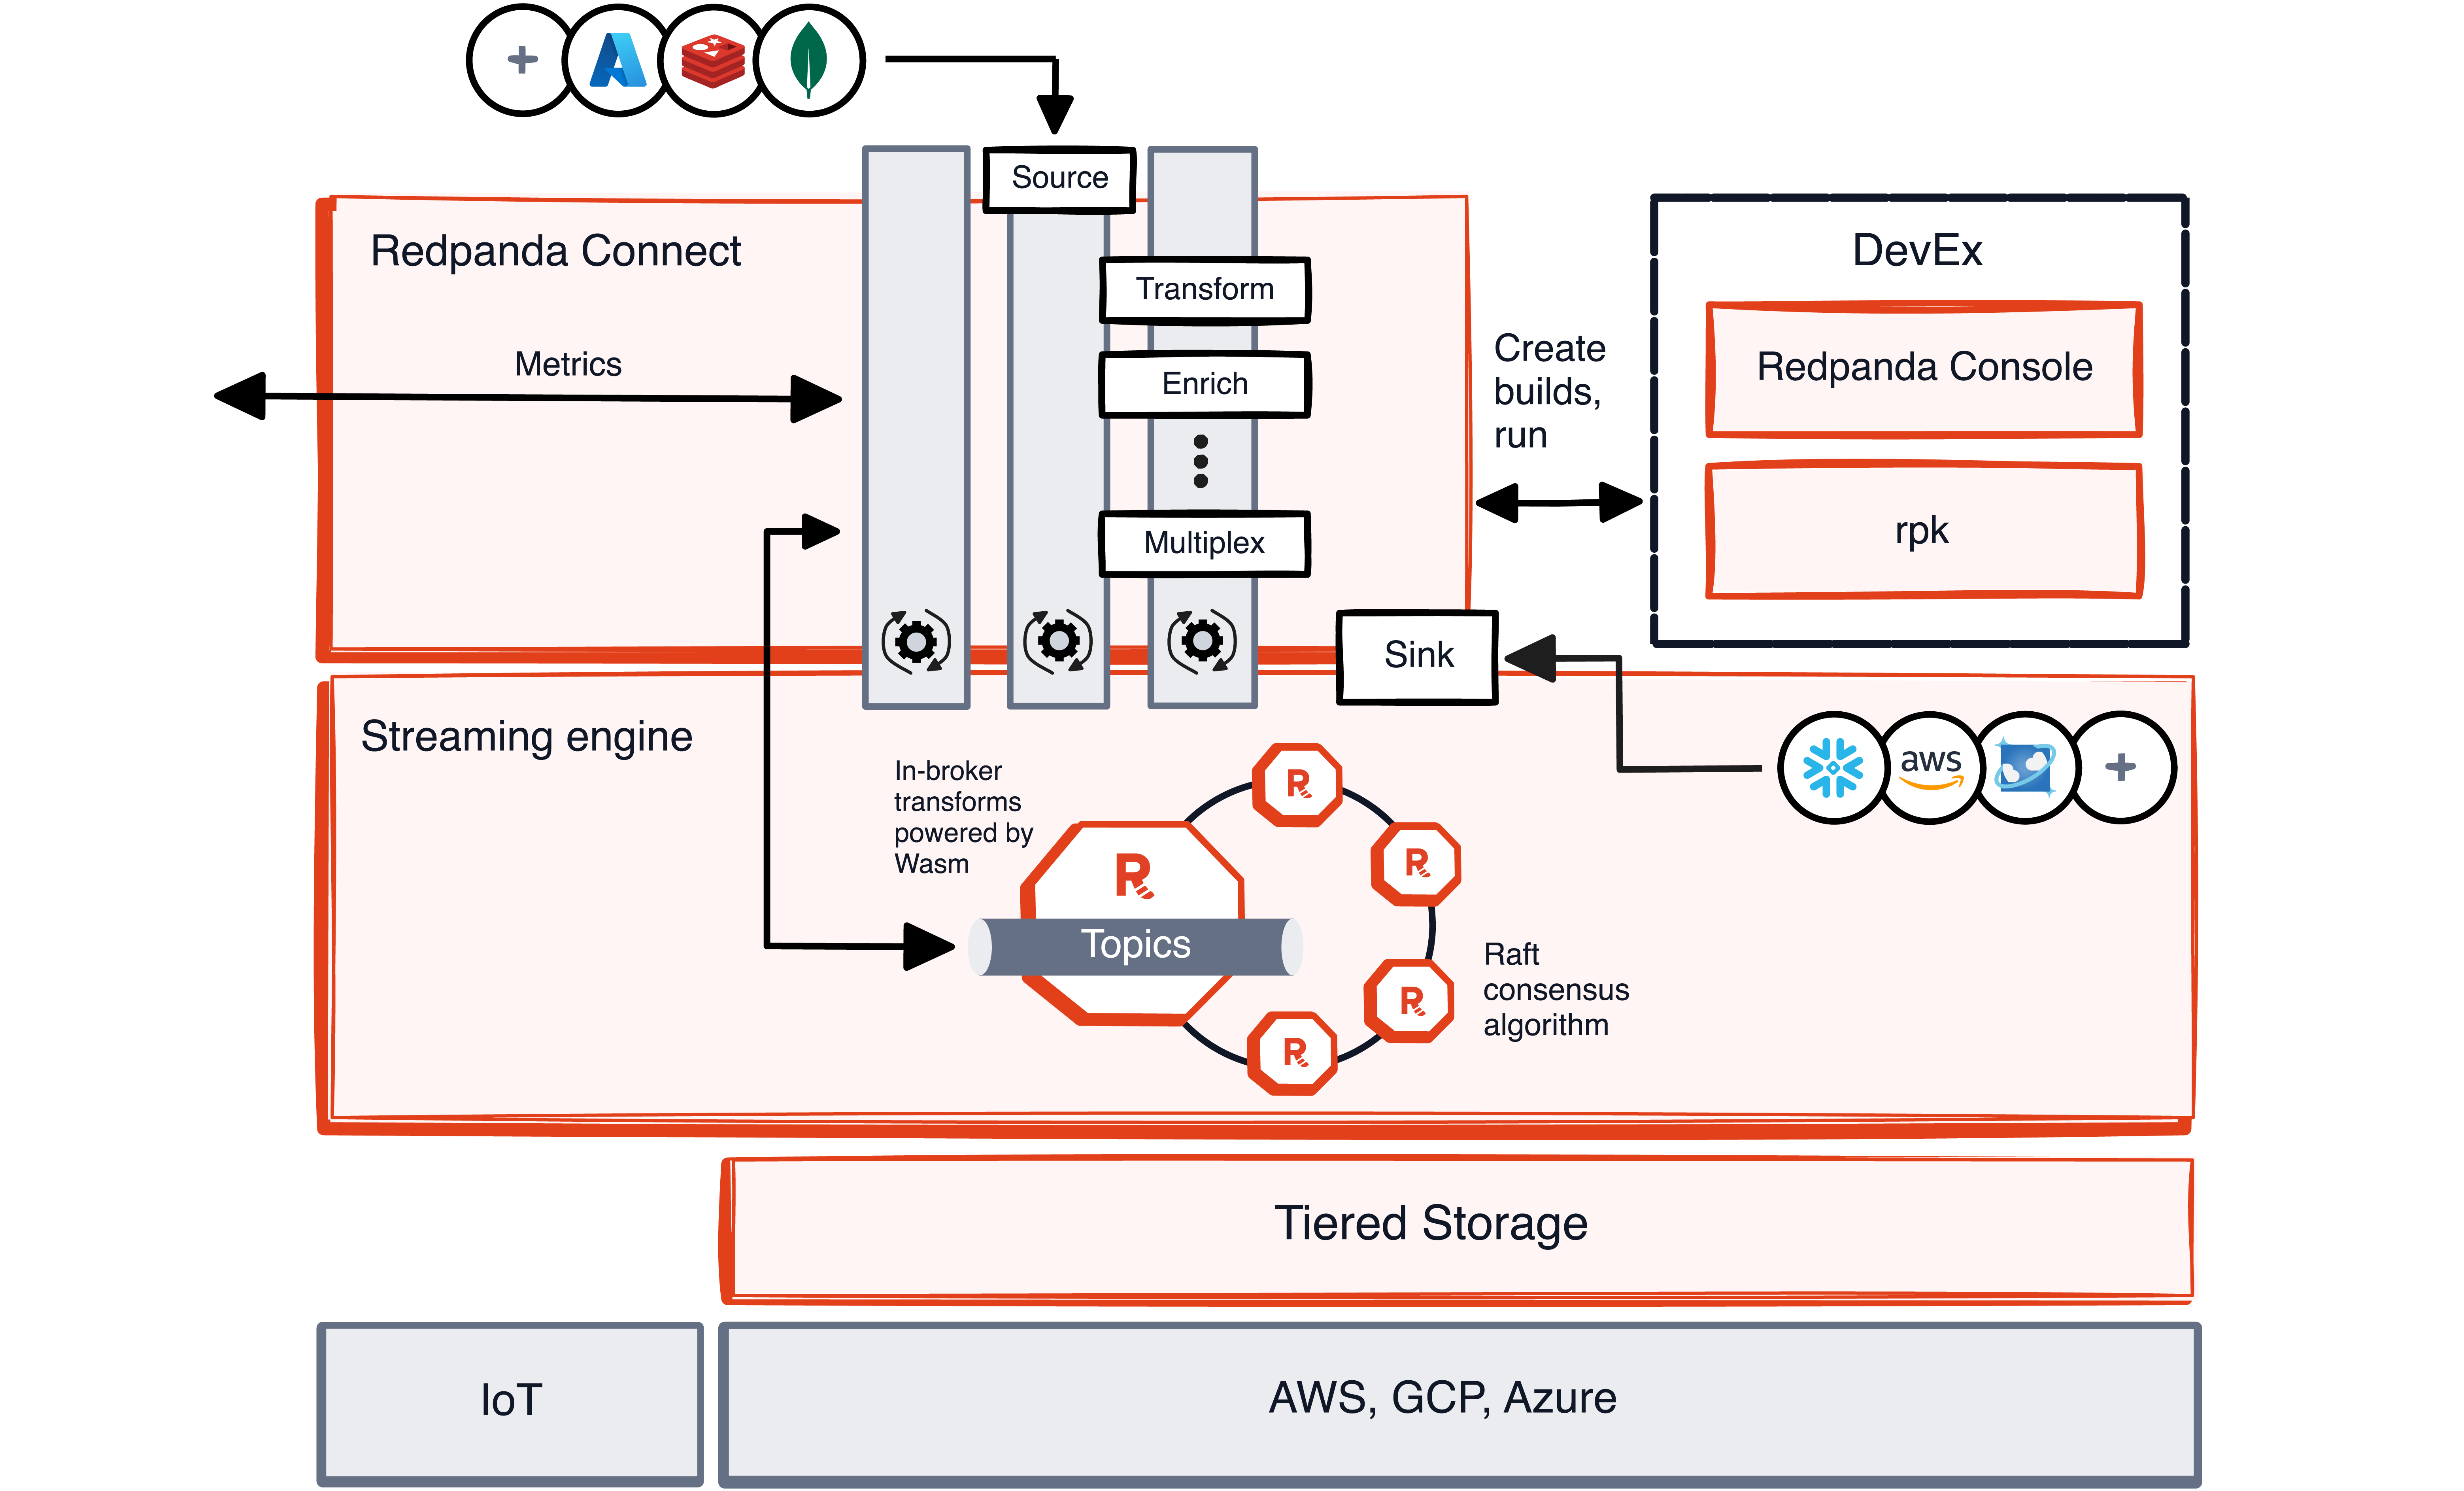
\includegraphics[width=0.8\textwidth]{resources/chapter-2/redpanda.png}
    \caption{Apa itu Redpanda? \parencite{whatIsRedpanda}}
    \label{fig:what-is-redpanda}
\end{figure}

Redpanda merupakan \textit{event streaming platform} alternatif dari Apache Kafka. Selain itu, platform ini menawarkan kompatibilitas API yang sama dengan Kafka sehingga memudahkan migrasi penggunanya. Meskipun begitu, terdapat beberapa perbedaan antara Redpanda dengan Apache Kafka.

Perbedaan pertama adalah algoritma konsensus yang digunakan. Apache Kafka menggunakan ZooKeeper (versi lama) sedangkan Redpanda menggunakan Raft. Meskipun begitu, versi terbaru Kafka sudah menggunakan algoritma konsensus Kraft yang merupakan varian dari Raft dengan perbedaan pada mekanisme replikasi log \parencite{raftKraft}.

Selain itu, Redpanda berfokus pada pengoptimalan kinerja yang lebih baik dibandingkan dengan Apache Kafka. Redpanda ditulis dalam bahasa C++, sedangkan Apache Kafka ditulis dalam bahasa Java dan berjalan pada JVM. Dalam hal ini, Redpanda menggunakan bahasa sistem sehingga minim \textit{overhead}.

Berikut adalah contoh pengoptimalan yang dilakukan pada Redpanda: \textit{Direct Memory Access (DMA)} untuk I/O, distribusi pemrosesan \textit{interrupt request} (IRQ) pada beberapa core CPU, penggunaan model \textit{thread per core}, dan pengoptimalan lainnya. Penggunaan model \textit{thread per core} memungkinkan Redpanda untuk menjalankan \textit{thread} aplikasi pada inti CPU yang sama sehingga \textit{context switching} dan \textit{blocking} dapat dihindari \parencite{redpandaArchitecture}.

\subsection{\textit{Change Data Capture}}

Menurut \cite{dataIntensiveApplications}, \textit{change data capture (CDC)} merupakan sebuah proses yang mengobservasi setiap perubahan pada data yang ditulis ke dalam basis data dan mengekstraknya ke dalam bentuk yang bisa direplikasi oleh sistem lain. Sebagai contoh, perubahan pada database bisa di-\textit{capture} lalu diterapkan pada \textit{search index} untuk menyamakan data pada basis data. Apabila \textit{log} diaplikasikan dalam urutan yang sama, data pada \textit{search index} dan basis data bisa dipastikan sama.

\begin{figure}[ht]
    \centering
    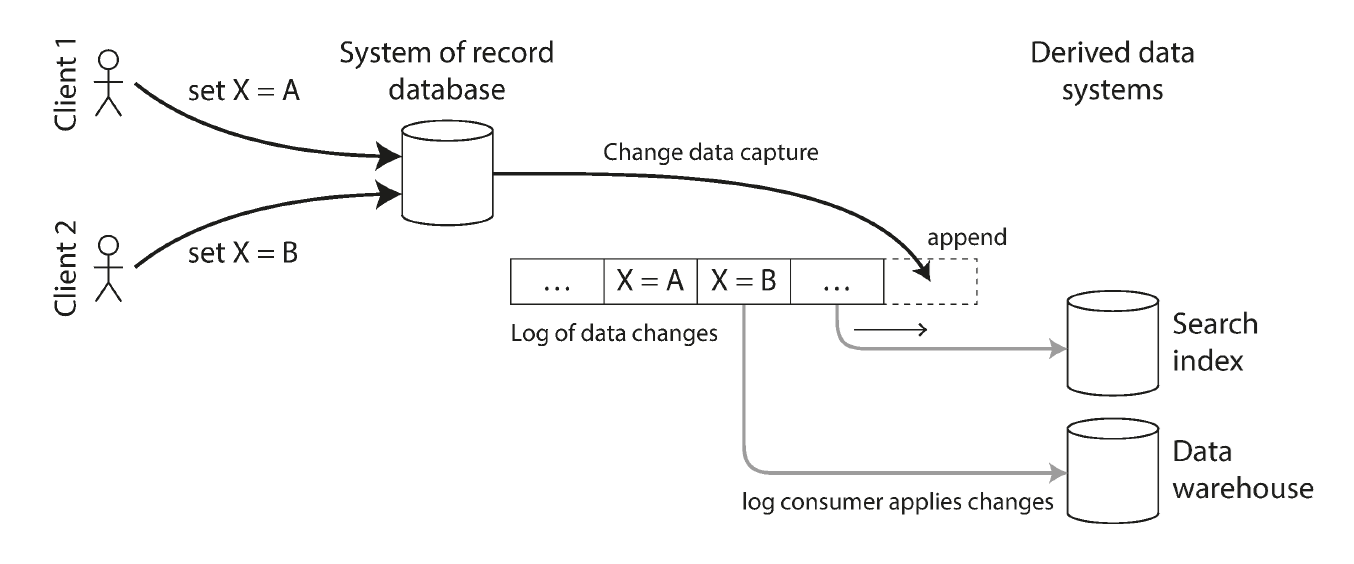
\includegraphics[width=0.8\textwidth]{resources/chapter-2/cdc.png}
    \caption{\textit{CDC Illustration \parencite{dataIntensiveApplications}}}
    \label{fig:cdc-illustration}
\end{figure}

PostgreSQL juga mendukung CDC dengan istilah \textit{logical replication}. Mekanisme ini menggunakan model \textit{publish} dan \textit{subscribe}. PostgreSQL yang mengirimkan \textit{log} bertindak sebagai \textit{publisher}, lalu terdapat \textit{subscriber} lain yang mengonsumsi \textit{log} yang dipublikasikan. \textit{Subscriber} ini bisa berupa replika PostgreSQL lagi atau aplikasi lainnya \parencite{pgLogicalReplication}. PostgreSQL mendukung dua mode operasi untuk replikasi, yaitu replikasi secara \textit{asynchronous} dan \textit{synchronous} \parencite{insideLogicalReplication}. Pada mode \textit{synchronous}, \textit{subscriber} harus merespons terlebih dahulu terhadap perubahan data sebelum PostgreSQL dapat melakukan \textit{commit}.

\begin{figure}[ht]
    \centering
    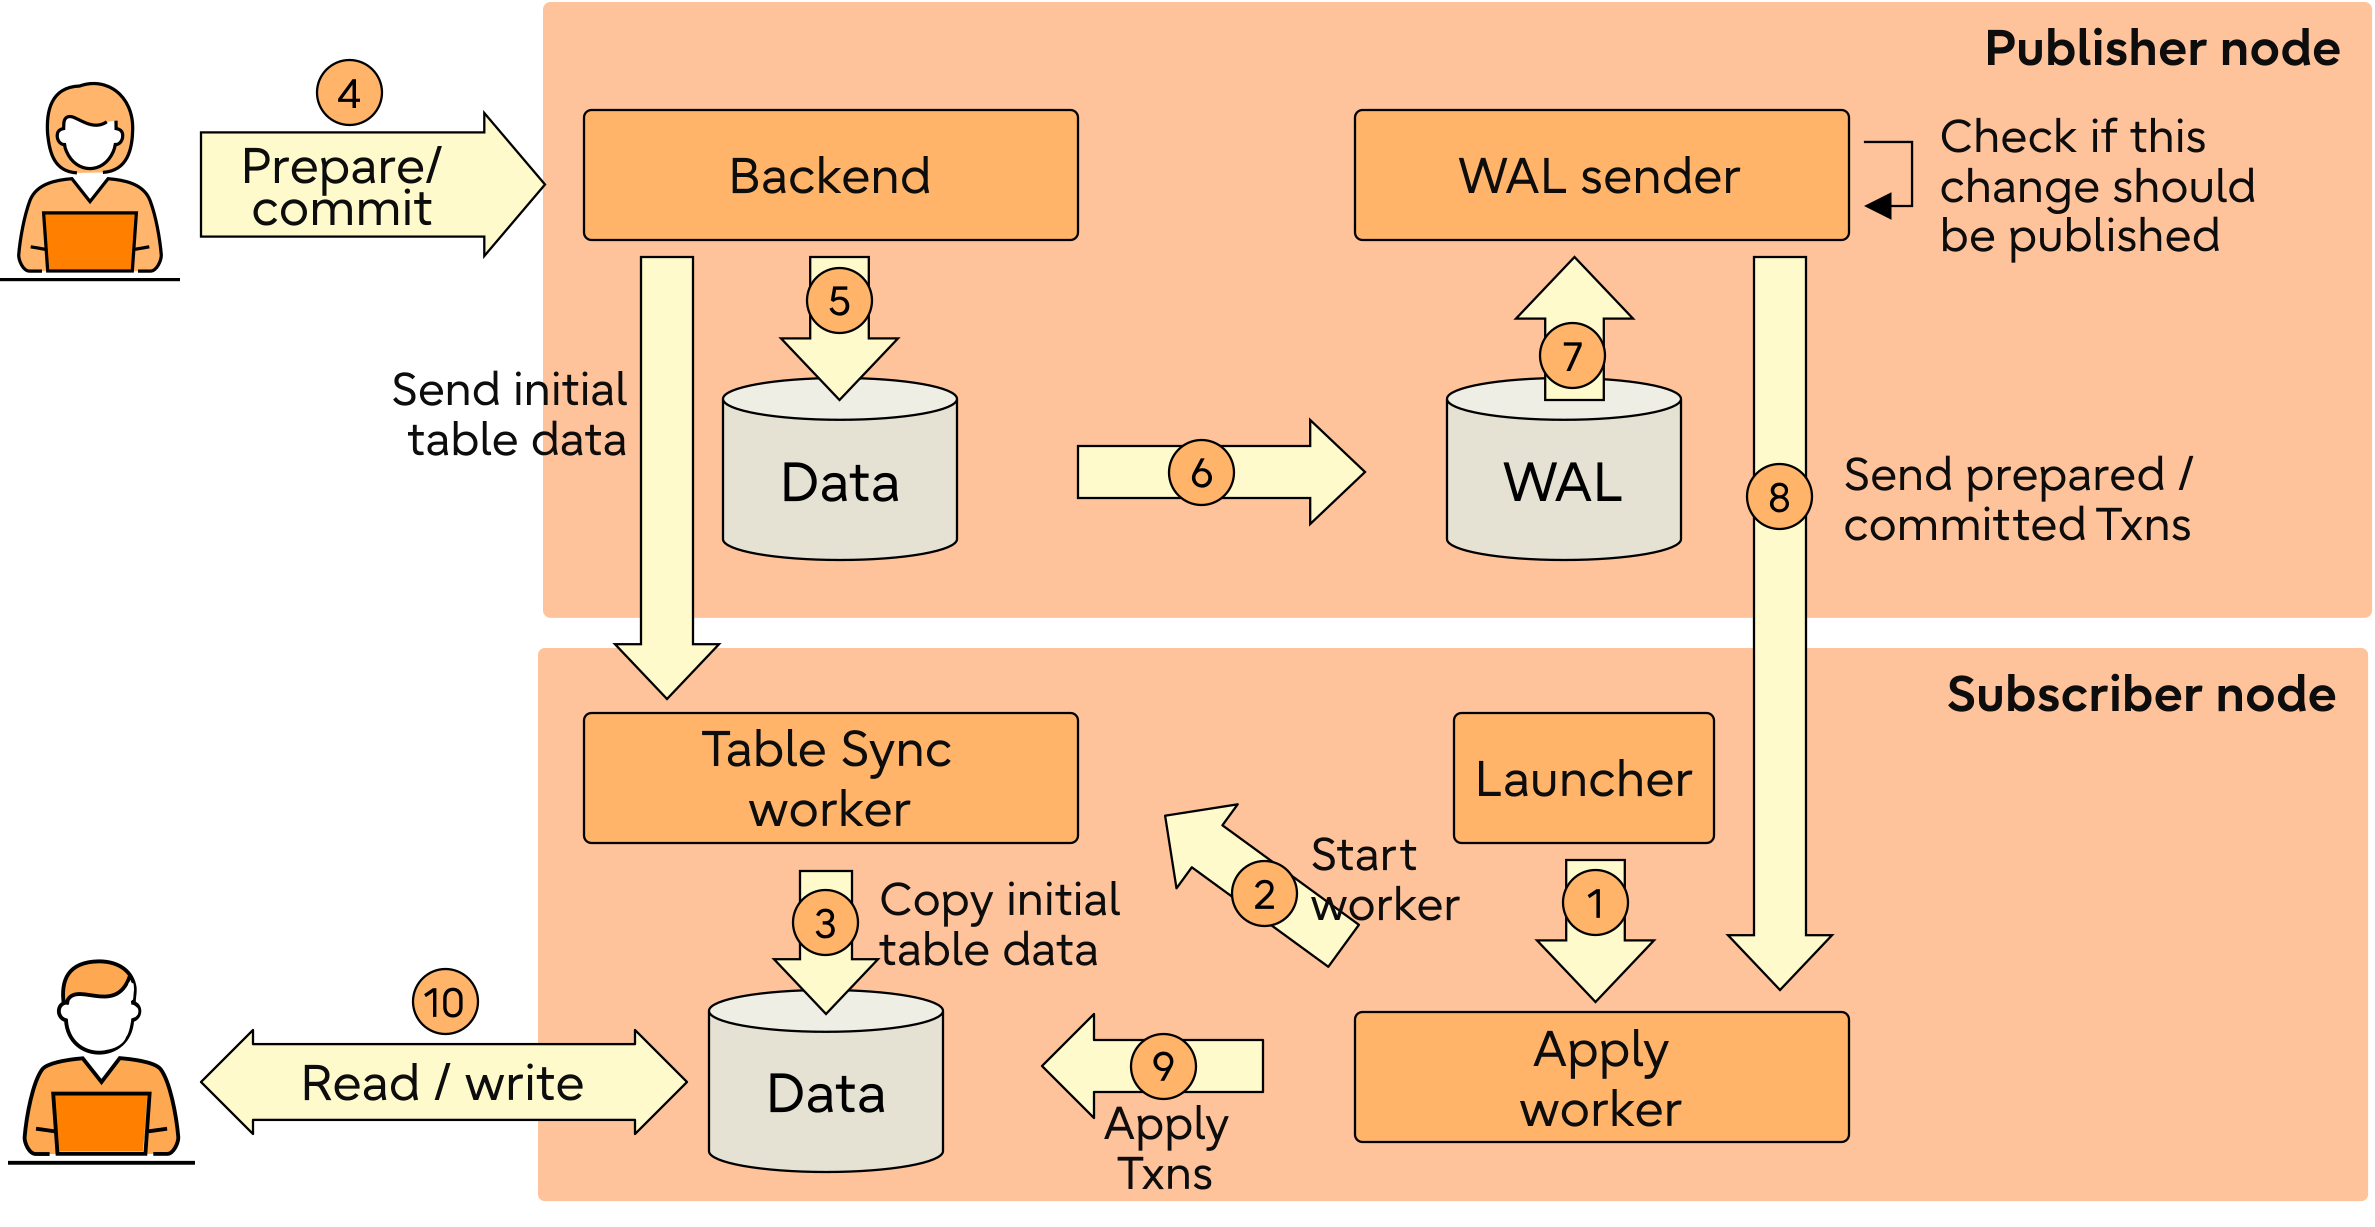
\includegraphics[width=0.8\textwidth]{resources/chapter-2/postgres-logical-replication.png}
    \caption{\textit{Logical Replication Architecture \parencite{insideLogicalReplication}}}
    \label{fig:logical-replication-architecture}
\end{figure}



\subsection{\textit{Event Sourcing}}

Mirip seperti \textit{change data capture}, \textit{event sourcing} juga menyimpan setiap perubahan pada \textit{state} aplikasi sebagai \textit{log of events}. Perbedaan terbesarnya terletak pada level abstraksinya. Pada \textit{change data capture}, aplikasi menggunakan basis data \textit{in a mutable way} dan dapat memperbarui atau menghapus \textit{record} sesuka hati. Aplikasi yang menulis pada basis data tidak harus \textit{aware} bahwa terdapat CDC. Berbeda dengan \textit{event sourcing}, logika aplikasi dibandung secara eksplisit di atas asumsi \textit{immutable event} yang ditulis pada \textit{event log}. Pada kasus ini, \textit{event} berupa \textit{append only}. Singkatnya, \textit{event sourcing} didesain untuk bisa merefleksikan hal yang terjadi pada level aplikasi dan bukan pada \textit{low-level state changes}.

\section{Pemrosesan \textit{Stream}}

Secara umum, \textit{stream} merujuk pada data yang tersedia secara inkremental dari waktu ke waktu. Konsep ini dipakai di berbagai tempat, seperti stdin dan stdout Unix, koneksi TCP, dan lain-lain \parencite{dataIntensiveApplications}.

\textit{Stream processing} merupakan paradigma pemrograman yang memandang \textit{stream} atau urutan \textit{event} sebagai objek masukan dan luaran utama dari komputasi. \cite{streaming101} menyatakan bahwa \textit{stream processing} merupakan tipe mersin pemrosesan data yang didesain dengan mempertimbangkan data yang tidak terbatas.

\cite{streamProcessingComparison} menyatakan bahwa terdapat karakteristik penting pada \textit{stream processing}, yaitu:

\begin{enumerate}
    \item \textit{Delivery guarantees}. Setiap informasi yang masuk harus dijamin akan diproses oleh \textit{streaming engine}.
    \item Toleransi kegagalan (\textit{fault tolerance}). Ketika terjadi kegagalan, \textit{streaming engine} harus mampu melakukan pemulihan dan memulai ulang dari titik yang ditinggalkan.
    \item \textit{State management}. \textit{Streaming engine} harus memiliki mekanisme untuk menyimpan dan memperbarui informasi \textit{state}.
    \item Memiliki kinerja yang baik dari sisi latensi, \textit{throughput}, dan skalabilitas.
    \item Memiliki fitur yang lebih canggih, seperti \textit{event time processing}, \textit{watermarks}, \textit{windowing}, dan lain-lain.
\end{enumerate}

Selain itu, karakteristik \textit{stream processing} juga bisa dibagi menjadi dua jenis, yaitu:

\begin{enumerate}
    \item \textit{Native streaming}. \textit{Stream processing} jenis ini akan langsung memproses data yang diterima secepat mungkin. Contoh \textit{stream processing} tipe ini adalah Apache Storm, Apache Flink, Apache Kafka Streams, dan Apache Samza.
    \item \textit{Micro-batching}. \textit{Stream processing} jenis ini meproses data setiap beberapa detik atau milidetik sekali sehingga data diproses dalam setiap kelompok kecil dengan sedikit keterlambatan. Contoh \textit{stream processing} tipe ini adalah Apahe Spark Streaming dan Apache Storm-Trident.
\end{enumerate}

\subsection{RisingWave}

RisingWave merupakan \textit{cloud-native streaming database}. Setelah menghubungkan sumber \textit{stream}, pengguna dapat membuat kueri analisis dengan mendefinisikan \textit{materialized view}, yang diperbarui secara inkremental pada RisingWave \textit{streaming engine} \parencite{risingwave}.

Berikut adalah keuntungan RisingWave:

\begin{enumerate}
    \item Mudah dipelajari karena merupakan ekstensi dari sintaks PostgreSQL.
    \item Mudah dioperasikan dan memiliki kebutuhan sumber daya yang lebih rendah karena ditulis dalam bahasa sistem Rust.
    \item Mendukung berbagai sumber data dan mampu mengirimkan (\textit{sink}) data ke dalam berbagai sumber, seperti mengambil data dari Apache Kafka lalu hasilnya dikirim ke ClickHouse. RisingWave mendukung integrasi dengan PostgreSQL CDC dan Apache Kafka sebagai sumber (\textit{source}) dan tujuan data (\textit{sink}).
    \item Menjamin konsistensi pada \textit{materialized view} dengan menggunakan \textit{snapshot}.
\end{enumerate}

\begin{figure}[ht]
    \centering
    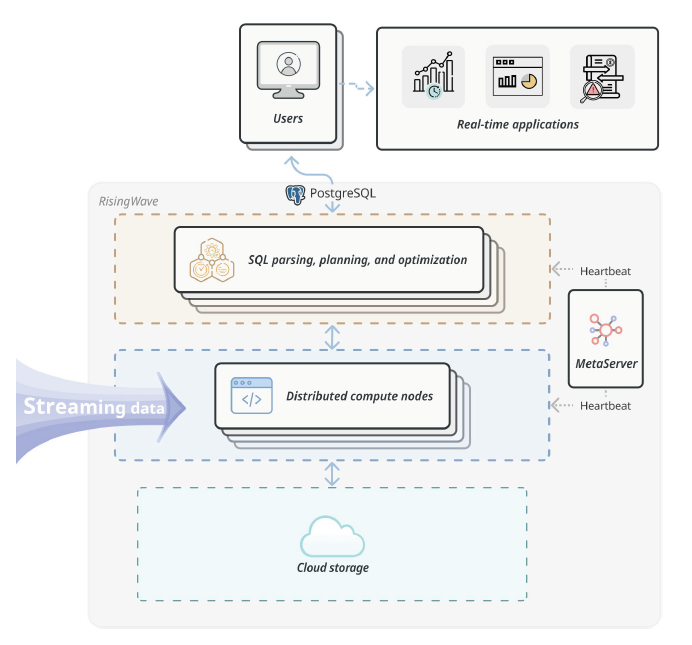
\includegraphics[width=0.8\textwidth]{resources/chapter-2/risingwave.png}
    \caption{Arsitektur RisingWave \parencite{risingwave}}
    \label{fig:risingwave-architecture}
\end{figure}

Node komputasi pada RisingWave terdiri atas \textit{batch engine} dan \textit{streaming engine}. \textit{Batch engine} meliputi \textit{query execution engine} dan \textit{exchange service} untuk menukar data antar node komputasi. \textit{Streaming engine} dibangun atas model aktor pada pemrograman konkuren. Mesin ini berinteraksi langsung dengan \textit{frontend} dan melayani \textit{stream data}. Selain itu, terdapat \textit{meta service} yang berperan sebagai layanan sentral untuk menyimpan metadata seperti keadaan kluster, katalog sistem, keanggotaan kluster, dan lain-lain \parencite{risingwave}.

\section{Pola Penyeimbangan Beban Berbasiskan Antrean}

Sebuah layanan dalam satu sistem seringkali bertugas untuk mengerjakan sesuatu dan memanggil layanan lain. Dalam kasus ini, terdapat kemungkinan munculnya masalah kinerja dan keandalan ketika layanan mengalami beban yang tinggi. Keadaan ini dapat menciptakan situasi \textit{backpressure}.

Dalam konteks perangkat lunak, \textit{backpressure} dapat didefinisikan sebagai \textit{resistance or force opposing the desired flow of data through software} \parencite{backpressureExplained}. Selain melakukan penyesuaian pada sumber daya sistem, terdapat tiga strategi yang dapat digunakan untuk menangani \textit{backpressure}, yaitu:

\begin{enumerate}
    \item Mengurangi kecepatan produsen mengirimkan pesan.
    \item Menggunakan \textit{buffer} untuk sementara mengakumulasikan pesan.
    \item Membuang (\textit{drop}) sebagian pesan yang diterima.
\end{enumerate}

Pola penyeimbangan beban berdasiskan antrean (\textit{Queue-based load leveling}) merupakan pola desain yang menyelesaikan masalah \textit{backpressure} dengan menggunakan antrean yang bertindak sebagai \textit{buffer} antara pesan dengan sebuah layanan, sehingga beban dapat dikontrol dan layanan tetap berjalan dengan stabil \parencite{queueLoadLeveling}.

\begin{figure}[ht]
    \centering
    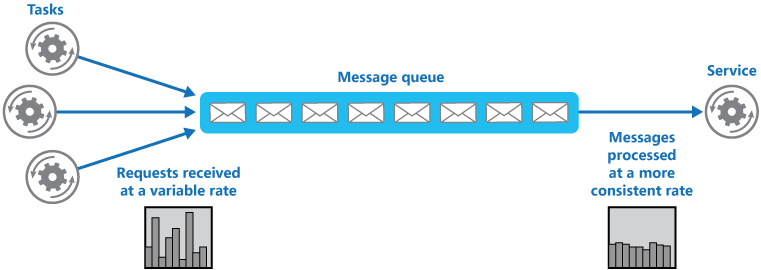
\includegraphics[width=0.8\textwidth]{resources/chapter-2/queue-based-load-leveling-pattern.png}
    \caption{Contoh Pola Penyeimbangan Beban Berbasiskan Antrean \parencite{queueLoadLeveling}}
    \label{fig:queue-based-load-leveling-pattern}
\end{figure}

Penggunaan antrean memisahkan pesan dengan pekerja, sehingga pekerja dapat menangani pesan berdasarkan kemampuannya, terlepas dari banyaknya pekerjaan yang bertambah seiring dengan berjalannya waktu. Pola ini memiliki berbagai keuntungan, seperti menjaga ketersediaan, memaksimalkan skalabilitas, dan membatasi biaya atau penggunaan sumber daya. Meskipun begitu, penggunaan pola ini akan meningkatkan latensi, terlebih lagi apabila pesan yang dikirimkan jauh lebih besar daripada kapasitas pemrosesan pada sistem.

\section{Segregasi Tanggung Jawab Kueri dan Perintah}

Segregasi tanggung jawab kueri dan perintah (\textit{Command-Query Responsibility Segregation}, CQRS) merupakan sebuah pola yang memisahkan operasi baca dan tulis untuk sebuah media penyimpanan data. Dalam pemodelan data, seringkali model data yang sama digunakan untuk operasi pembacaan dan pembaruan. Meskipun begitu, seringkali kedua operasi tersebut memiliki kebutuhan yang berbeda. CQRS menggunakan model data yang berbeda untuk operasi yang berbeda. Selain itu, beban pekerjaan untuk kedua operasi tersebut seringkali asimetris dan memiliki kebutuhan kinerja dan penskalaan yang berbeda \parencite{msCQRS}.

Perintah (\textit{command}) merupakan pesan yang berfokus pada pekerjaan, seperti "pesan kamar hotel" dibandingkan dengan "ubah status reservasi suatu kamar menjadi sudah dipesan". Dengan pendekatan ini, perintah dapat diproses secara asinkron.

\begin{figure}[ht]
    \centering
    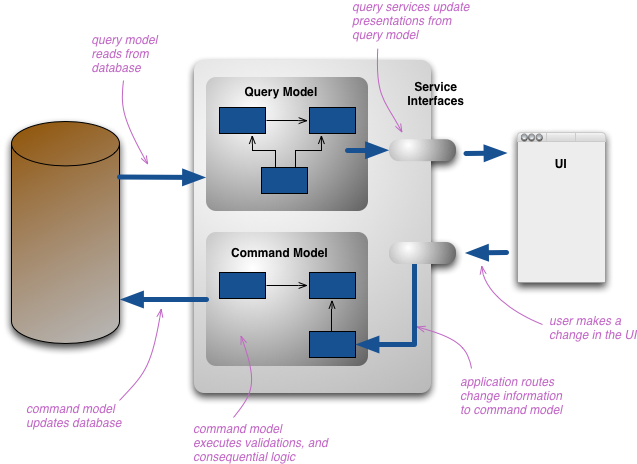
\includegraphics[width=0.8\textwidth]{resources/chapter-2/cqrs.png}
    \caption{Ilustrasi CQRS \parencite{fwCQRS}}
    \label{fig:cqrs-illustration}
\end{figure}

Pendekatan ini memungkinkan pemisahan data untuk operasi baca dan data untuk operasi tulis. Pembacaan data dapat dilakukan pada skema atau basis data yang telah dioptimalkan untuk operasi tersebut, seperti menyimpan data di memori, \textit{materialized view}, atau pun yang lainnya.

Pendekatan ini memungkinkan penskalaan secara independen dan \textit{separation of concerns}. Meskipun begitu, implementasinya bisa menjadi kompleks dan apabila basis data untuk operasi pembacaan dan penulisan berbeda, data menjadi \textit{eventual consistent}.

\section{\textit{Key-Value Store}}

\subsection{Redis}

Redis (Remote Dictionary Service) merupakan basis data \textit{open-source} berbasiskan \textit{key-value store}. Redis mendukung berbagai tipe data, mulai dari string, bitmap, bitfield, hash, list, set, hingga stream. Selain itu, Redis merupakan basis data yang menyimpan data pada memori (\textit{in-memory}) dan berjalan secara \textit{single thread} sehingga Redis berjalan dengan cepat dan tidak perlu memikirkan konkurensi. Selain itu, Redis memiliki banyak dukungan fitur seperti dukungan \textit{persistence} dengan \textit{snapshot} atau \textit{append-only file} (AOF), dukungan \textit{high-availability}, replikasi, \textit{sharding}, \textit{pubsub}, \textit{stream}, dan lain-lain \parencite{redisExplained}.

\begin{figure}[htbp]
    \centering
    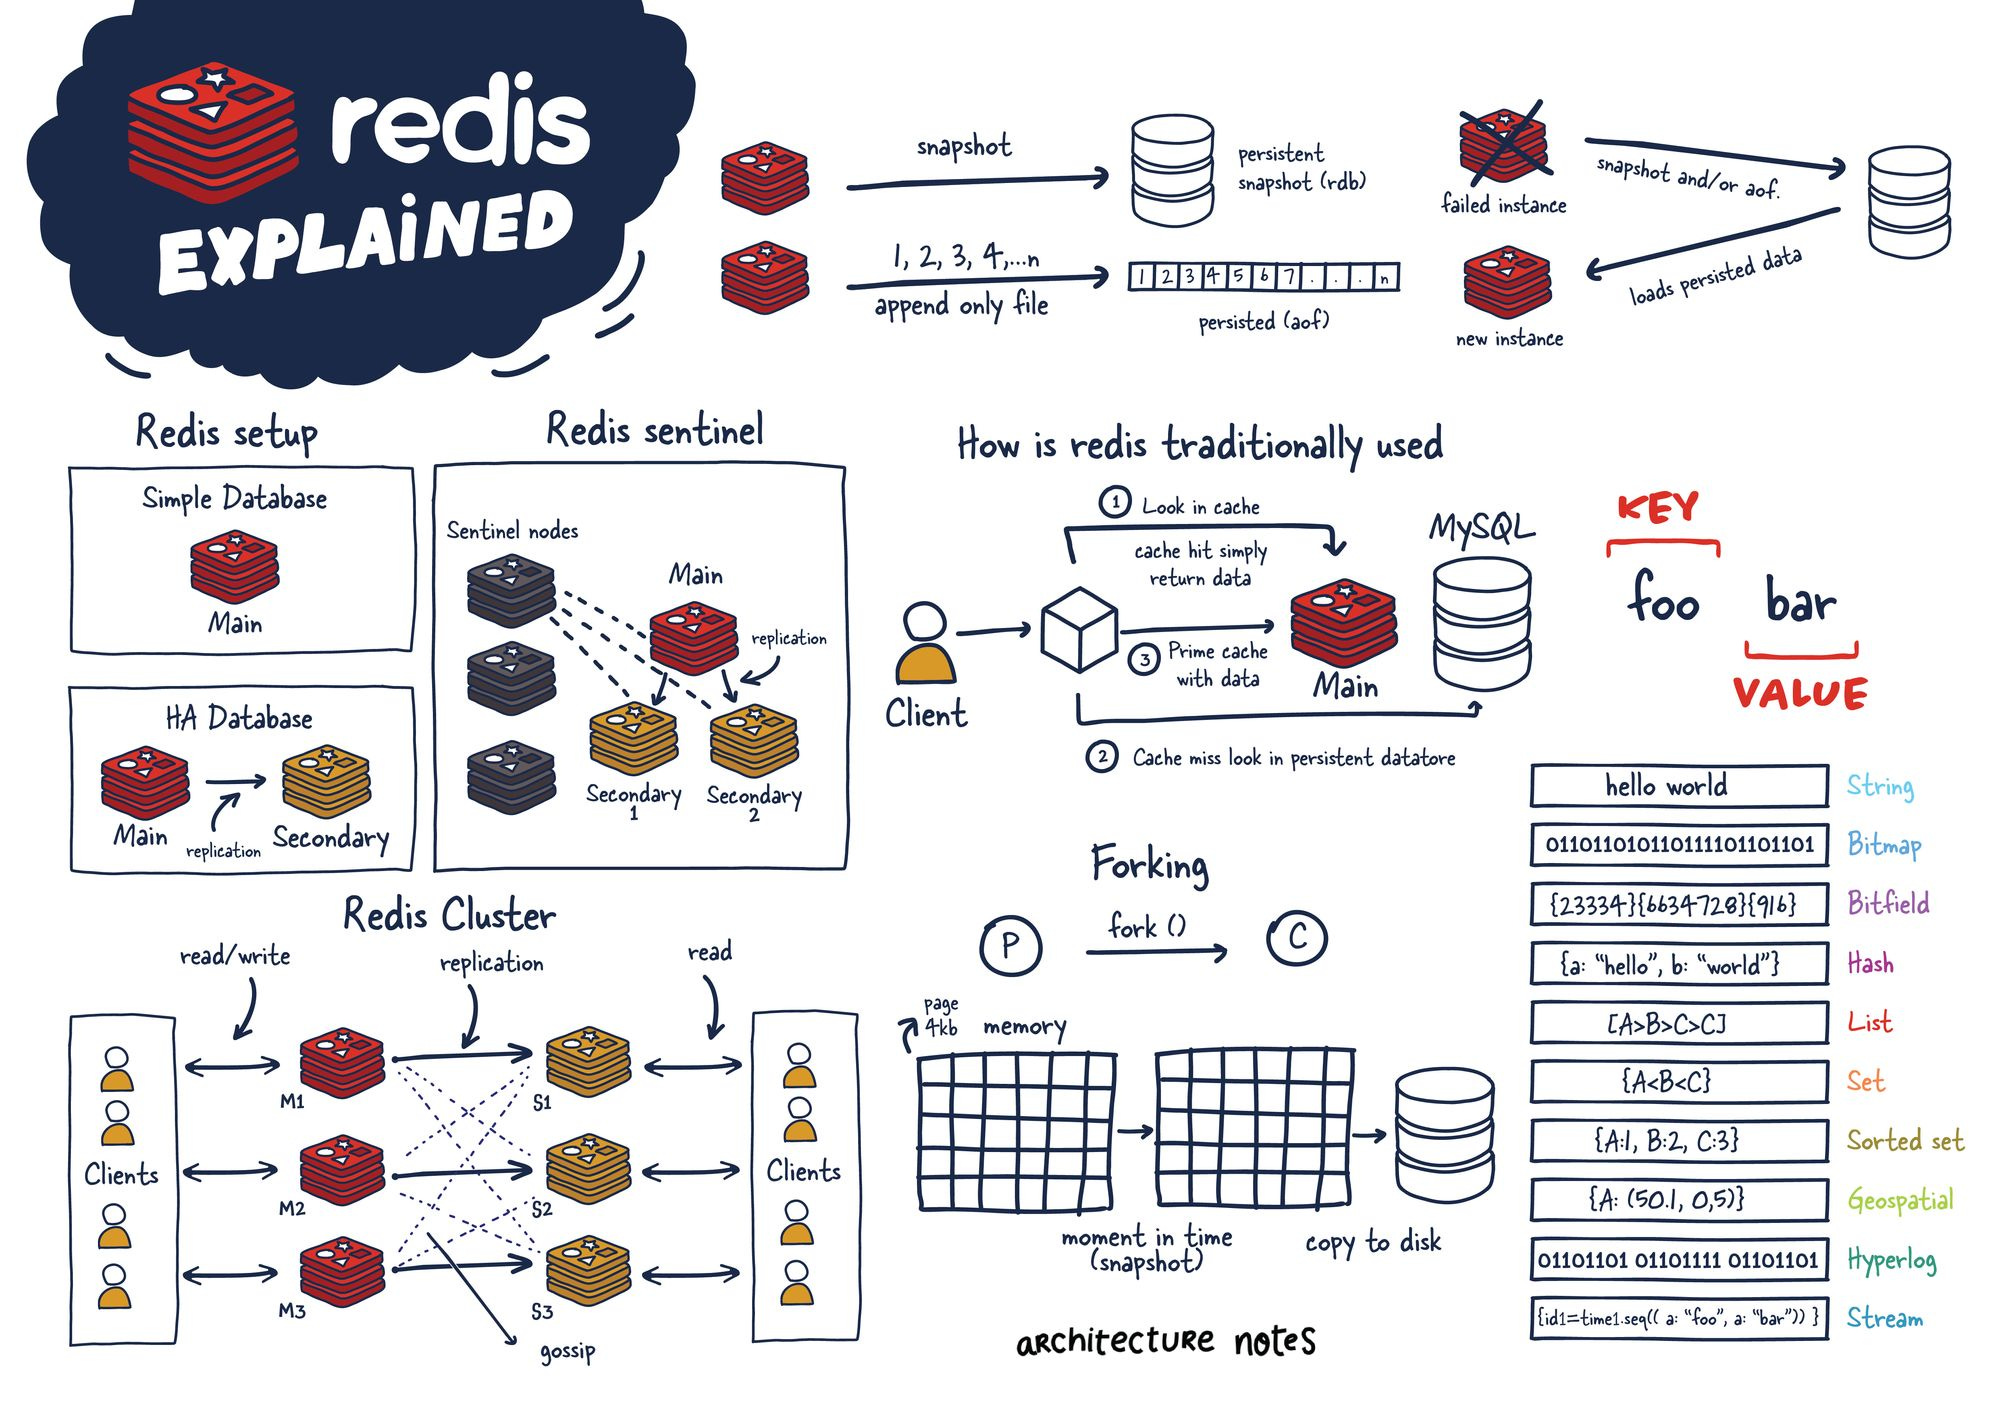
\includegraphics[width=1\textwidth]{resources/chapter-2/redis.jpg}
    \caption{\textit{Redis Explained \parencite{redisExplained}}}
    \label{fig:redis-explained}
\end{figure}

Konfigurasi Redis Cluster memungkinkan penskalaan secara horizontal dengan menyebarkan data pada mesin (\textit{sharding}). Redis menggunakan fungsi hash deterministik untuk mendistribusikan data. Selain itu, Redis menggunakan \textit{gossip protocol} untuk menilai keadaan kluster. Ketika \textit{master} tidak responsif, node \textit{secondary} dapat dipromosikan menjadi node \textit{primary} \parencite{redisExplained}.



\section{Penelitian dan Riset Terkait}

\subsection{Implementasi Arsitektur \textit{Microservices} Menggunakan Komunikasi \textit{Event-Driven} Pada Aplikasi Pemesanan Tiket Acara (Jeeves)}

Tugas akhir ini membahas aplikasi pemesanan tiket acara dengan arsitektur \textit{microservice} dengan komunikasi berbasis peristiwa. Tujuan dari penelitian tersebut adalah membuat aplikasi tiket yang tahan akan kegagalan sehingga layanan yang masih berjalan tetap dapat memenuhi aksi yang lain. Untuk itu, arsitektur \textit{microservice} diimplementasikan dengan cara \textit{loosely-coupled}. Agar hal tersebut dapat dipenuhi, komunikasi berbasis peristiwa digunakan. Agar ketergantungan antar layanan berkurang, seluruh data yang diperlukan oleh sebuah layanan diikutsertakan pada peristiwa yang dikirim \parencite{microservicesEventDriven}.

\begin{figure}[htbp]
    \centering
    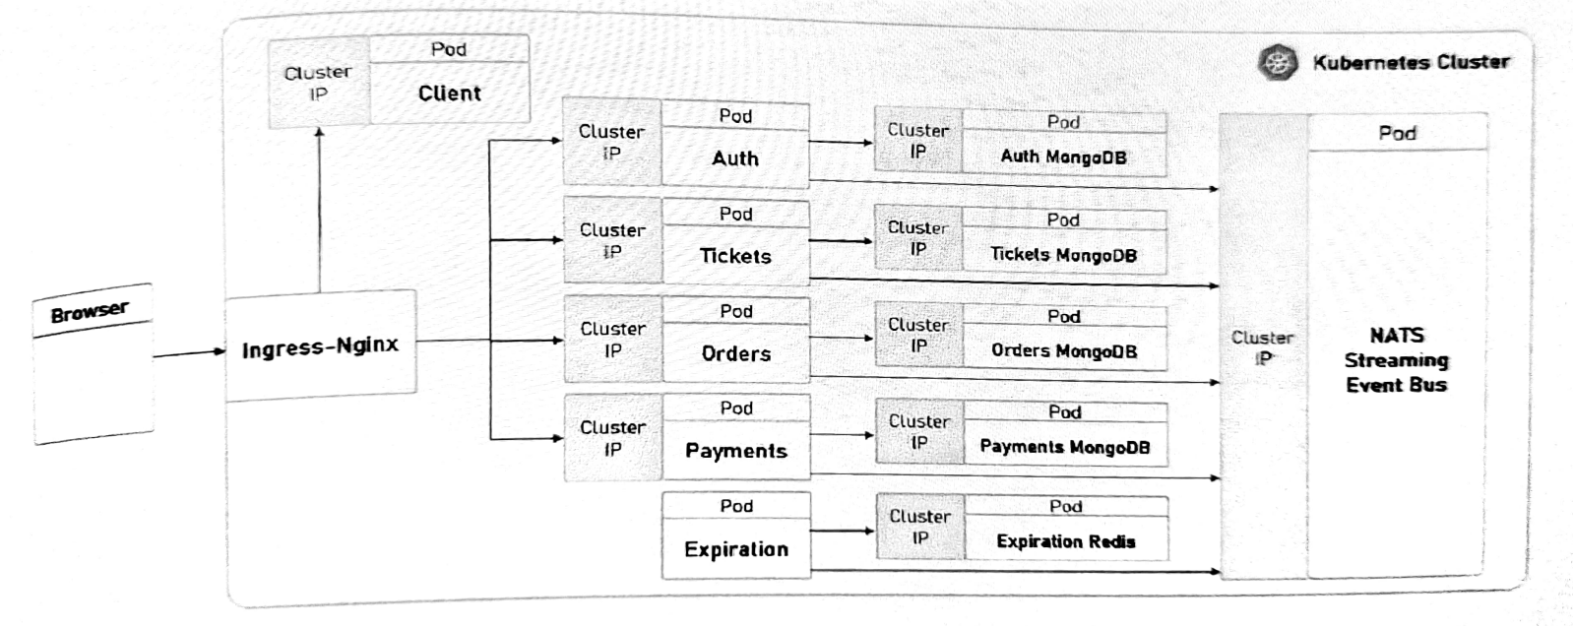
\includegraphics[width=1\textwidth]{resources/chapter-2/jeeves.png}
    \caption{Arsitektur Jeeves \parencite{microservicesEventDriven}}
    \label{fig:jeeves-architecture}
\end{figure}

Penelitian ini mengimplementasikan fungsionalitas dasar seperti otentikasi pengguna, pembuatan tiket, reservasi tiket, dan pembayaran tiket. Terdapat lima \textit{microservice} yang dibuat, yaitu layanan otentikasi, layanan tiket, layanan pemesanan, layanan pembayaran, dan layanan kadaluarsa. Setiap layanan selain layanan kadaluarsa memiliki basis data masing-masing dengan menggunakan MongoDB. Hanya layanan kadaluarsa yang menggunakan Redis. Selain itu, setiap komunikasi yang terjadi secara asinkron dilakukan melalui NATS. Untuk melakukan validasi otentikasi, sistem ini menggunakan JWT dengan rahasia bersama yang diatur oleh Kubernetes. Pendekatan ini memungkinkan layanan independen terhadap layanan otentikasi \parencite{microservicesEventDriven}.

Penelitian ini berhasil mengimplementasikan arsitektur aplikasi untuk pemesanan tiket acara yang tahan kegagalan dengan pendekatan \textit{microservice} dan berbasis peristiwa. Meskipun begitu, penelitian ini tidak membahas dan menguji aspek skalabilitas dan elastisitas dari sistem ini.

\subsection{\textit{Backend for a Ticketing System}}

Tesis ini membahas desain \textit{backend} untuk sistem tiket. Tesis ini berfokus pada desain modul, fungsionalitas, serta relasi yang diperlukan untuk menjalankan sistem ini. Penelitian ini berbeda dengan penelitian sebelumnya yang fokus membahas desain dari sisi arsitektur. Tesis ini tidak membahas arsitektur secara detil dan hanya membagi fungsionalitas menjadi beberapa modul. Oleh karena itu, arsitektur yang digunakan pada penelitian ini adalah arsitektur \textit{modular monolith}. Selain itu, penelitian ini memakai prinsip REST API dalam mendesain implementasi API \parencite{backendForTicketing}.

Terdapat empat entitas yang digambarkan pada sistem ini, yaitu:

\begin{enumerate}
    \item Pengguna yang bertugas untuk mencari dan membeli tiket, melakukan pembayaran, dan mengubah profil pengguna.
    \item Organisasi yang bertugas untuk mengatur acara, kategori tiket, dan lain-lain.
    \item Validator yang bertugas untuk memberi izin dan mencegah terjadinya pelanggaran yang berkaitan dengan validitas dan integritas tiket.
    \item Admin yang bertugas atas registrasi organisasi dan mengatur sertifikat penjual tiket.
\end{enumerate}

Figur \ref{fig:event-rm} dan \ref{fig:ticket-storage} menggambarkan diagram relasi entitas untuk \textit{events} dan entitas yang berkaitan pada proses pembuatan dan penyimpanan tiket.

\begin{figure}[htbp]
    \centering
    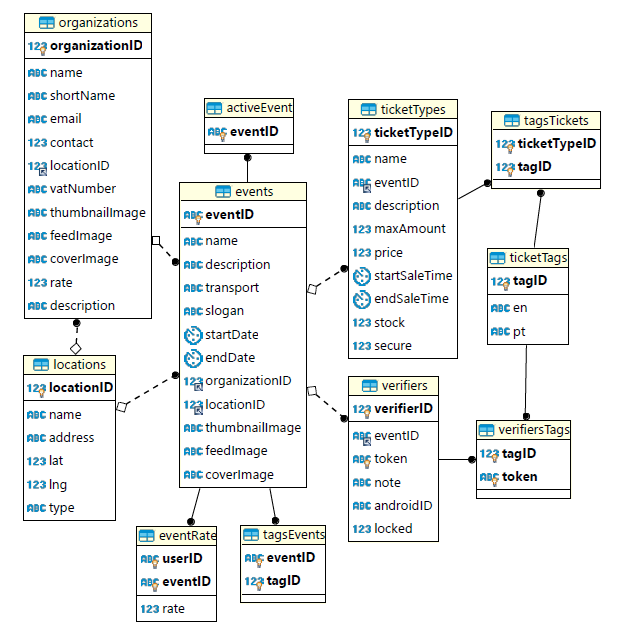
\includegraphics[width=0.6\textwidth]{resources/chapter-2/event-rm.png}
    \caption{ERD \textit{events} \parencite{backendForTicketing}}
    \label{fig:event-rm}
\end{figure}

\begin{figure}[htbp]
    \centering
    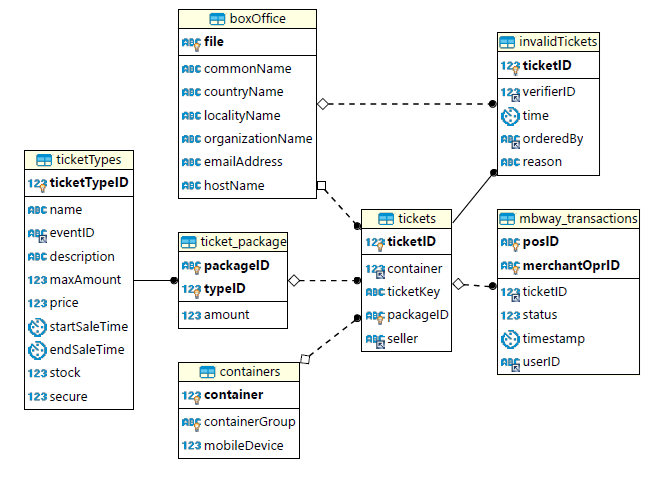
\includegraphics[width=0.6\textwidth]{resources/chapter-2/er-ticket-storage.png}
    \caption{ERD dengan entitas untuk pembuatan dan penyimpanan tiket \parencite{backendForTicketing}}
    \label{fig:ticket-storage}
\end{figure}

Sebagaimana dijelaskan sebelumnya, tesis ini hanya membahas sistem dari aspek desain fitur dan entitas. Arsitektur sistem tidak dibahas secara detil, sehingga kemungkinkan besar arsitektur yang diimplementasikan adalah arsitektur \textit{monolith}. Selain itu, aspek skalabilitas dan toleransi kegagalan tidak dibahas pada tesis ini.
